% !Mode:: "TeX:UTF-8" 

\BiChapter{绪论}{Introduction}\label{chap1}

%本章对 \LaTeX{} 排版系统做一个简要介绍,希望没有使用过 \LaTeX{} 的同学对 \LaTeX{} 有一个初步认识。

%=========================================================================================
\BiSection{研究背景与研究意义}{Research Background and Research Motivation}\label{chap11}
\BiSubsection{网络数据平面概述}{Network Data Plane Overview}\label{chap111}

%参考线性系统理论第一章的叙述方法,先要定义清楚研究对象。等等。。再看本文是否也能按照更好的方式叙述。

网络正以前所未有的速度越来越紧密地参与到民生社会中,为满足国家民生需求、新基建拉动内需和产业升级起到了至关重要的作用。从“百度一下”到网红全民直播带货,从实现“三网通”到发展“新基建”的国家战略,小到优化社会资源效率的办公数字化,大到勾勒出智能交通、智慧城市和万物互联的5G海洋,无一不是构建在网络基础设施的快速发展之上。思科公司预计,到2023年全球家用互联网总带宽将达到$5.85$Ebps\footnote{1 Ebps=$10^6$Tbps=$10^{18}$bps} (是现在的3.27倍),移动互联网用户预计达到57亿,其总流量可达$11.3$Ebps (将达到目前的5倍),其中5G流量将占据移动互联网总带宽的76.5\%(0.6\%,2019年)\citeup{huawei2019,cisco2019}。
由于深度学习、AI、大数据、云计算、物联网的快速发展\citeup{gubbi2013internet,hashem2015rise},这些新技术将催使新零售、新金融、新医疗、新教育、新制造、云视频和云游戏等行业“云化”,海量的数据会在数据中心内部服务器间网络以及外部网关中传递,这些关键应用将会改变数据中心算力构成和数据中心内部网络结构特性。

随着云服务概念和大规模机器学习的落地,以云计算为代表的数据中心网络规模成指数增长。同时,众核CPU架构快速发展,服务器内虚拟机布置资源大幅扩张,促使主机出口吞吐量从40GbE向100GbE甚至400GbE演进。此外,复杂的网络安全规则、流量监控等功能模块进一步吞噬了大量宝贵的CPU计算资源。
%设备统一化有助于降低网络部署的复杂度,研究人员通常需要持续进行网络测量、监控、容错、提升效能的工作。
为应对以上纷繁复杂的网络功能需求,近年来网络数据平面架构的发展尤为迅速\citeup{li2019hpcc,singh2015jupiter,alizadeh2010data,wu2012tuning}。传统网络以TCP/IP协议为核心,主要目标为增强网络扩容能力,主要展现了网络强大的敏捷性与自治能力。但当网络规模进一步增加,网络中容易出现广播风暴、链路收敛慢等问题。大型的核心网交换设备往往需要具有能够应对各种复杂应用场景的能力,这使得网络设备结构越来越复杂、设备内的功能众多而应用场景单一,最终导致了设备成本高昂、设备内程序运行资源浪费巨大的问题。
由于研究的创新和技术的推进,设备厂商不断开发出具备各种高级功能的交换芯片,硬件功能强大的同时,复杂的网络管理也遇到新的挑战。

“可编程网络”概念为网络架构带来了统一透明的控制接口,以及方便敏捷的网络管理能力。
作为可编程网络的先驱,软件定义网络(Software Defined Network,SDN\citeup{mckeown2008openflow})概念首次在2008年被斯坦福大学提出,其将大学校园网内交换设备的控制平面抽离出来,以增强网络管理配置灵活度以及网络的快速排错能力。到目前为止,世界各国都投入大量资源进行软件定义网络的技术研究与开发。2010年,阿里巴巴云网络飞天系统在大规模和低成本的要求下,利用SDN技术提高云网络的可靠性和使用弹性。2013年,Google公司的全球数据中心骨干网使用SDN技术将网络链路的利用率从75\%提升至99\%\citeup{jain2013b4}。2015年至今,阿尔卡特朗讯在欧洲建立了Nuage\cite{nuagenetworks}项目,主要旨在运营商、银行以及数据中心内部署SDN方案以增强网络基础设施的性能以及开发便捷性。2016年,中国盛科网络技术公司领导研发的“支持软件定义网络千兆以太网交换芯片”通过了由中科院院士、“核高基”专家、电信专家在内的鉴定委员会评审,旨在制造中国具有全球领先技术的可编程网络解决方案\citeup{centec}。2019年,中国联通通信公司完成国内首个基于SDN的互联网智能差异化服务商用部署,以应对4K/8K视频、VR、云应用等业务等对网络提出的多元化需求\citeup{liantongsdn}。对于网络节点数量大的复杂通信网络而言,集中控制可以有效地解决分布式信息同步缓慢,大规模网络问题排查困难等问题\citeup{zhang2016mind,zhang2018foces}。可编程网络的概念从学术到商用落地,均展现了它强大的技术优势以及产业界广泛的认同。


\BiSubsection{网络可编程技术}{Network Programmable Technology}\label{chap112}


如图~\ref{fig:networksdn}~左部所示,按照网络转发设备的功能划分,可将网络设备从逻辑上分为“控制平面和数据平面”。传统网络架构中,一般将数据平面与控制平面集中在一起组成完整的设备。根据组网需求的不同,开发人员将同类型的网络设备互相连接在一起。每个设备内的控制平面会按照事先规定的协议算法与邻居节点或远端节点进行通信,同步完消息之后,每个设备节点都会拥有全局的网络拓扑数据,并在数据平面内安装根据路径选择好的转发策略。然而,当网络节点数量增加,网络拓扑连接变得复杂之后,传统的网络架构会面临网络拓扑信息共享速度缓慢等问题。同时,由于控制平面内均构建了自主运行的控制算法,网络管理员无法及时获取设备中实时的运行状态,对于当网络中出现任何问题时,开发人员很难精准定位故障点。此外,传统网络架构的核心交换机或路由器中,通常搭载了完整功能的软件算法,使得设备可以适应各类场景,但通常一个设备的运行周期之内,设备并不会频繁更换拓扑连接,也不会随意中断运营业务,这就造成了设备功能臃肿与制造高成本之间的矛盾。综上所述,传统网络设备的软件代码量庞大,生态闭塞、难以快速增加新的功能,灵活性低、不具有可编程性,因此急需要一种新的网络体系架构,来解决传统网络可扩展性差的不足之处。

\begin{figure}[!ht]
	\centering 
	\vspace{-1.5mm} 
	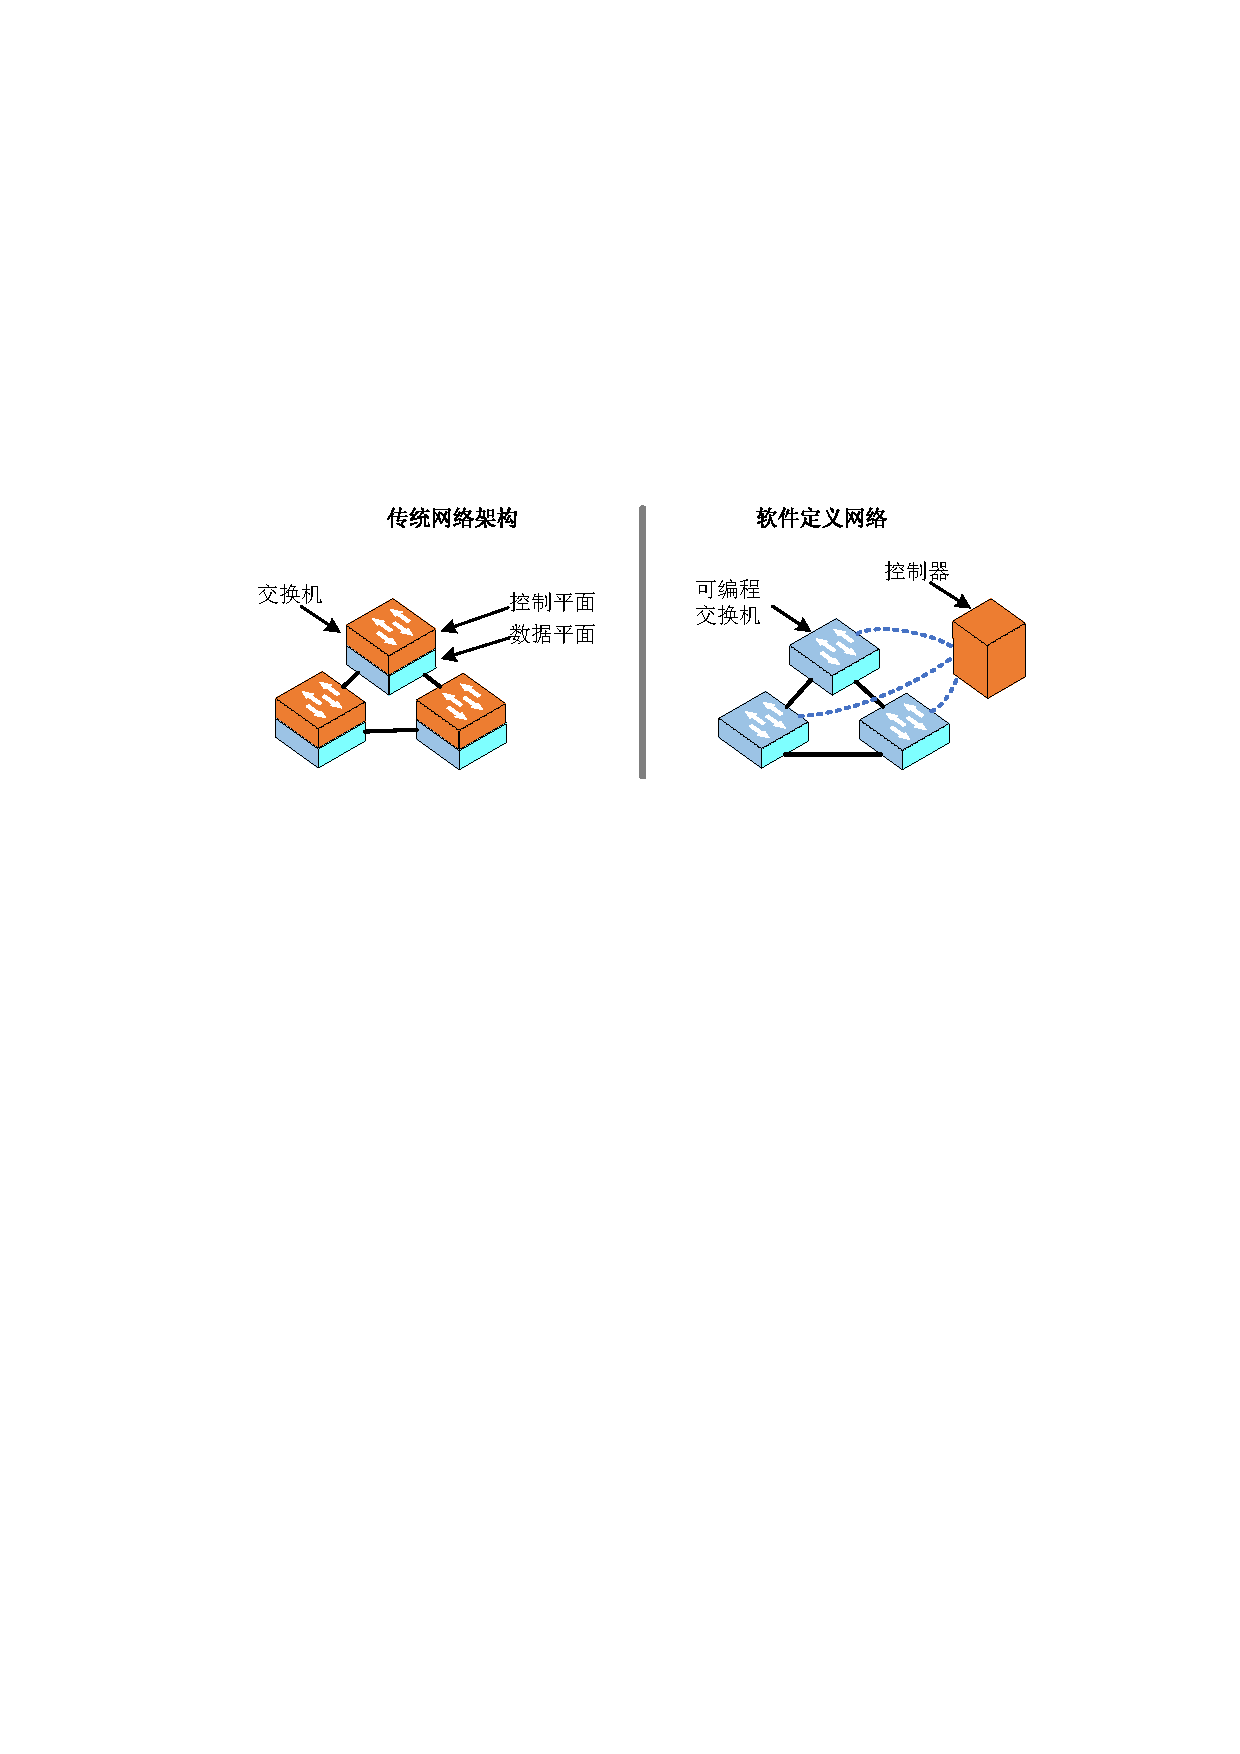
\includegraphics[scale=1]{networksdn.pdf}
	\caption{传统网络与软件定义网络架构比较} \label{fig:networksdn}
\end{figure}

作为可编程网络的重要组成部分,软件定义网络(SDN)技术(图~\ref{fig:networksdn}~右侧所示)将网络设备中的SDN将数据平面和控制平面解耦\citeup{mckeown2008openflow,ethane}。在数据平面上,对数据包的处理统一做查找-转发(Match-Action)抽象。控制平面负责建立网络拓扑,控制并下发流表。这样所有的数据包转发行为都由控制平面的软件逻辑管理,数据平面的设计将变得统一并且简单。由于软件具有强大的灵活性以及开发的敏捷性,SDN大大加速了网络创新和智能化管理的进程。OpenFlow\citeup{mckeown2008openflow}协议已经是数据平面和控制平面的通讯桥梁的事实标准,并由安全通道(Secure Channel)构成。
SDN网络的数据平面趋于统一化、简单化,是用于完成计算机之间通信数据包的匹配、修改、传送、转发的软硬件设备,厂商只需生产符合OpenFlow控制协议的白盒交换机,则设备可以被编程为适用与各种场景的状态。

\begin{figure}[!ht]
	\centering 
	\vspace{-1.5mm} 
	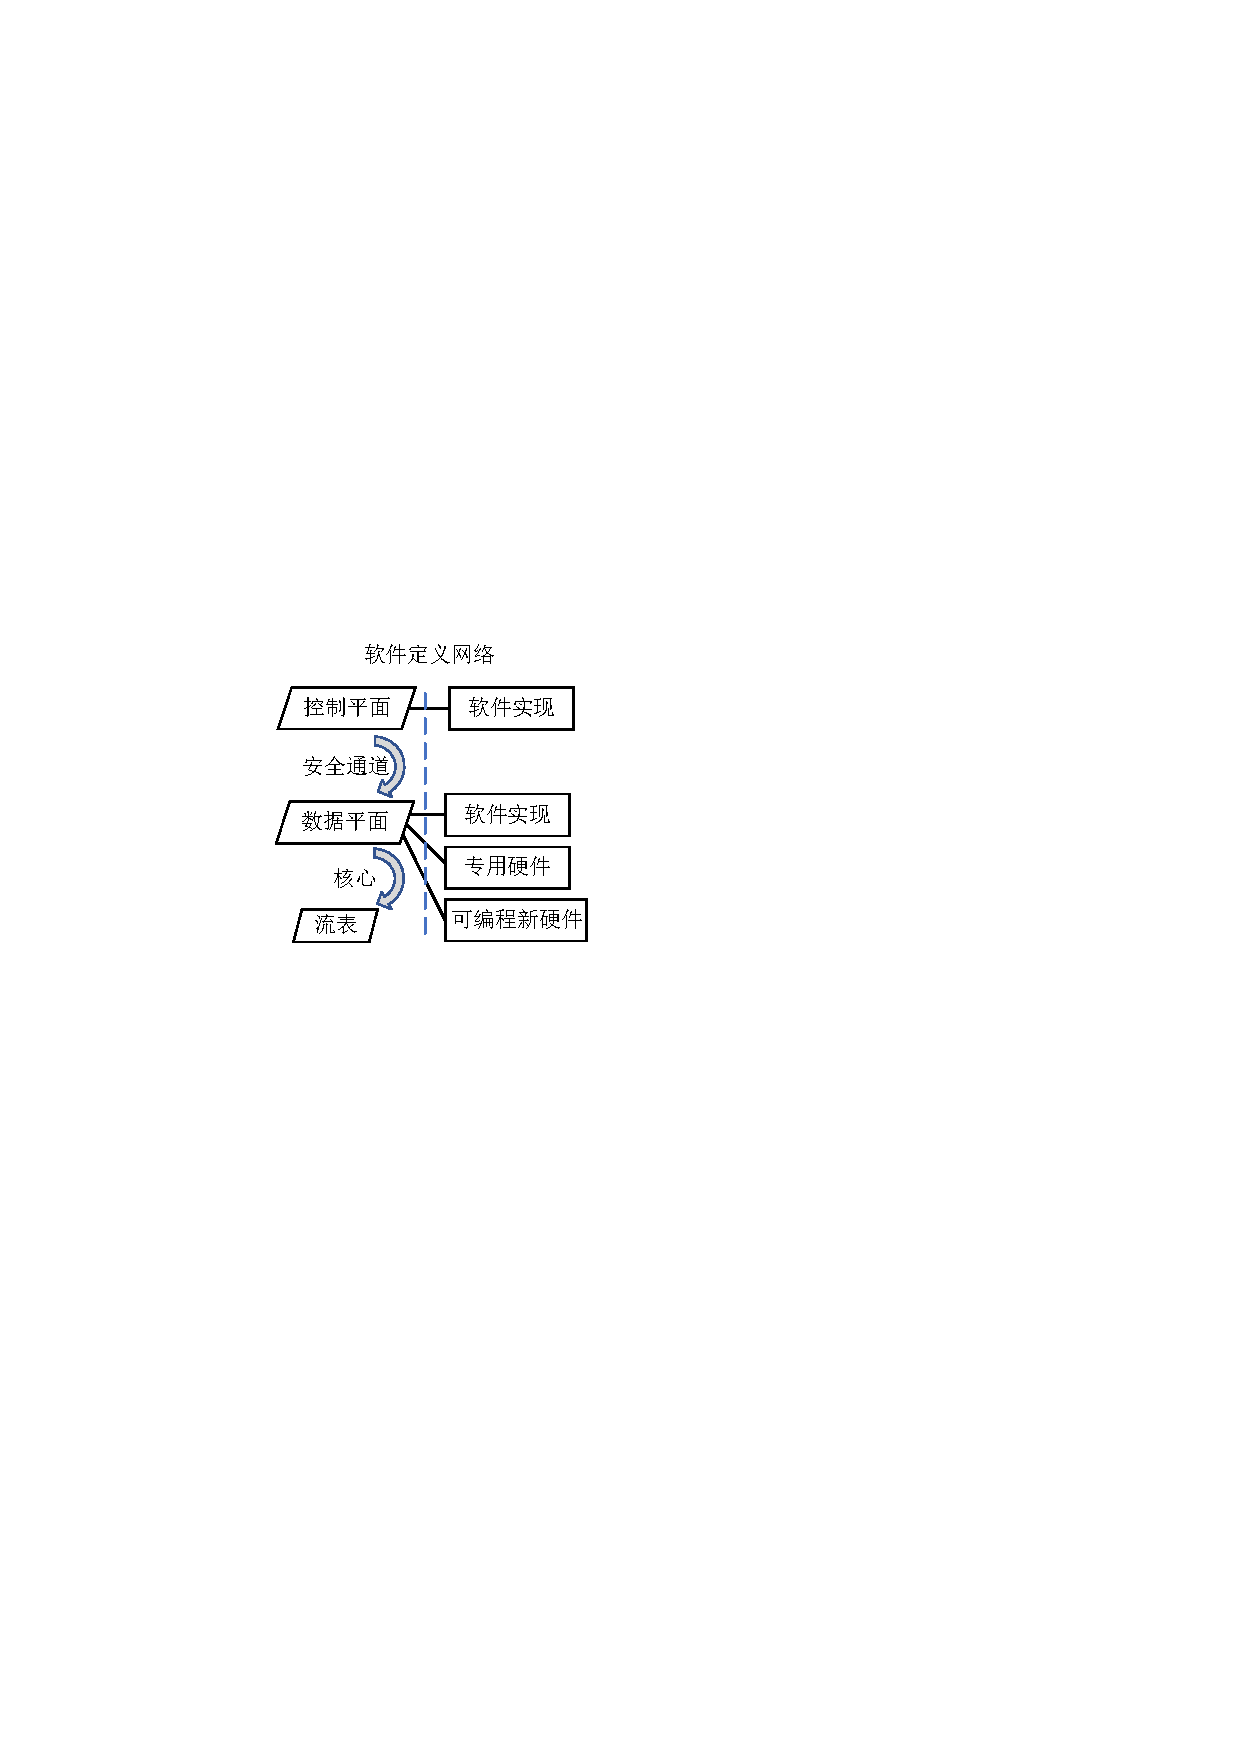
\includegraphics[scale=1]{sdnarcs.pdf}
	\caption{软件定义网络实现方案设计} \label{fig:sdnarcs}
\end{figure}

%软件定义网络的基本设计概念是将数据平面与控制平面分离。
	

数据平面的可编程性核心依赖于流表及其配置操作,网络管理员拥有对数据平面的各个特性做快速个性化定制的能力。
网络的控制平面维护全网视野、调度、配置针对流的转发条目。
运行在控制平面内的各种应用构成了其全部功能。
当前SDN网络系统设计架构如图~\ref{fig:sdnarcs}~所示,在不同场景下,网络对数据通信的需求千差万别,根据应用场景流量大小不同、处理过程复杂程度来设计选取数据平面的实现方案,目前主要有软件、专用硬件和新型可编程硬件等实现方案。
两者在功能上都能够对数据包做一系列处理,包括匹配、查找、统计、传送、转发和安全校验等,其中“流表”是实现数据平面功能的核心函数(器件)。数据平面包含一个可以与远端控制器沟通的代理机构,这部分功能着重于协议通信以及安全通道信息加解密,主要由轻量级处理器构成。

硬件交换机之于软件交换机的主要区别在于处理数据包的性能以及交换容量。数据包处理性能主要参数为吞吐量(字节每秒)和包吞吐量(包每秒)。目前基于软件实现的数据平面性能可达到60Gbps/60Mpps\citeup{pisces}。当数据包处理复杂度(操作步骤数量)增加时,软件交换机的性能会大幅下降。专用硬件交换机有接口数目多、交换容量大的特点,一般能满足64个100G端口的总交换容量。而且硬件交换机转发时延低,性能与数据包处理步骤数目几乎无关,稳定性良好。在核心网络和高性能网关等领域主要使用基于硬件的交换设备,但成熟设备功能固定、更换成本高,如果需要更新网络功能,几乎无所适从。所以目前在数据中心网络的NFV(网络功能虚拟化)等场景内,软件交换机依然占据很大份额。由于软件交换机灵活性高,开发人员能够快速迭代部署新功能,且传统单机通信速率需求不高,软件交换机尚能满足需求。但随着人工智能、5G领域的发展,数据中心网络内通信容量需求快速增长,转发时延收紧,软件交换机性能瓶颈凸显。运营商不得不为网络任务大量堆叠服务器。本文主要侧重于研究服务器和核心交换网络中,如何使用可编程硬件来大大缓解网络性能瓶颈。针对控制平面,本文使用SDN全局优化的思想,实现对网络中的瓶颈资源(如流表资源)的可扩展性并提升通信协议的安全性。



随着创新需求的进一步提高,只有让底层硬件拥有灵活的可配置能力才能满足目前行业变革的需求,因此研究人员提出了数据包处理编程协议无关(Programming Protocol-Independent Packet Processors,P4\citeup{p4})概念。如果说SDN给出了控制层的全局视野,那么协议无关可编程的数据平面给出了设备层的全局视野。SDN已经将数据平面高度抽象,操作人员可以灵活地定义数据流,以及对这种流进行怎样的操作。但是在数据平面内数据包头的匹配域却是预先规划好的。固有转发平面的设计思想会引起如下两个问题:其一,添加新特性需要跟业界讨论、以及等待很长的设备研发时间;其二,在数据平面内固化现实中可能出现的每一个网络协议字段造成宝贵计算资源的巨大浪费。满足新阶段的网络创新需要具有比SDN概念更好的灵活性、动态性。因此斯坦福大学提出了P4\citeup{p4}编程语言框架,这种语言有能力重新定义数据平面的包解析模式。P4源代码通过前端编译器编译为中间表示层代码,这个编译过程将提出源代码中的语义逻辑。之后需要根据不同的目标器件再进行后端编译,这个过程最终会生成目标器件对应的机器码,硬件可直接读取。目前P4的目标设备已经有基于ASIC的交换芯片、CPU、GPU和FPGA等多种实现。

P4扩展了可编程抽象的灵活性,包括可编程的包头域抽取器,以及可编程的多级流表。P4同时规范了一种编程语言\citeup{p4},它可以控制数据平面对数据包的任意解析行为,也可以自由配置查找表的数据位宽和多级流表之间的查找流水线\citeup{rmt,mswitch}。这种更高阶的硬件编程模型使交换设备更加透明,设备与网络协议解绑。除此之外,网络端到端的大带宽、低时延需求引申出了网络功能硬件卸载、网络随路计算等概念,这也进一步促使网络面向全面可编程化方向发展。
协议无关处理器从诞生至今已经覆盖了广泛的网络应用场景:
1)替代传统网元(服务负载均衡\citeup{miao2017silkroad}、安全控制\citeup{lapolli2019offloading}、流量控制\citeup{yang2018elastic}、测量\citeup{kim2015band}),使云网络自身成为一个软硬任务分配均衡且可编程的系统。
2)增加网络随路专用功能,如键值查询(key-value store)\citeup{jin2017netcache}。旨利用网络高速以及可编程交换机特点,使特殊功能的性能大幅提升。

P4规范的网络可编程数据平面可编程性依然比较弱,只能自主设定包头域以及匹配表,无法增加其他适应性计算。
在一些网络延时要求严苛的场景,网络随路计算概念应运而生,网络可编程性差也成了制约网络发展的关键因素。
编程灵活性,与吞吐性能是天平的两端,由于网络巨大的性能需求,很难同时获得很高的可编程性。在此之外,也有很多特性是P4架构无法实现的:
1)包头长度有限,目前数据平面可编程的流水仅仅紧局限于处理宽度受限的包头。
2)非图灵完全,只有有限个数的固化的“执行器”。
3)没有讨论包调度问题。
4)无法对数据包进行可编程的带状态处理。而这些问题目前被认为是因追求高性能而带来的设计折中\citeup{lec8rmtp4,chole2017drmt}。

\BiSubsection{可编程网络的关键问题}{Key Issues of Programmable Networks}\label{chap113}

复杂化的网络架构以及快速增长的数据包吞吐容量,对网络的管理方式以及可编程的配置能力都提出了巨大挑战。本文主要围绕计算机网络可编程化问题中的处理性能增强以及可编程灵活性提升等两个子问题进行了深入分析,可编程网络由软件定义网络概念引出,其将网络的分为了控制平面与数据平面。在优化数据平面处理灵活度时,又发展出了数据包协议无关处理器等概念,其可针对不同协议数据包的处理需求,灵活地在线升级数据平面的功能,从而追求提升数据平面的可用性。针对这两大研究领域,现有的可编程网络设计领域主要面临了以下三方面的问题:


\begin{itemize}
	\item {\hei 网络数据平面的运算资源问题}:转发设备中的流表是控制平面表达控制灵活性的关键运算资源。为了快速处理数据包,数据平面内部一般使用特殊的运算资源来降低每个数据包的处理耗时,例如使用快速存储器或硬件查找表,而这类专用运算资源一般会耗费较大的存储资源和制造成本。作为高性能网络内设备核心资源的流表因造价高、容量小导致网络内极易产生流表溢出等现象。随着网络数据包吞吐容量以及SDN网络对流表消耗量的快速提升,核心运算资源数量有限与其分配的供需矛盾问题日益凸显。
	
	
	\item {\hei 网络数据平面可编程能力问题}:虽然硬件交换机在网络性能方面大幅超越基于通用软件服务器的数据平面,但是基于白盒交换机和数据平面可编程专用芯片的编程能力受限。目前实现灵活网络功能主要依赖于全可编程平台构建的数据平面,包括基于CPU的通用软件处理平台、网络处理器以及可编程逻辑器件(FPGA)等。但真实环境中的包处理过程非常繁琐,现阶段可编程数据平面依然有着灵活性与性能之间的矛盾,全可编程平台处理效能极低,而且目前基于CPU的处理平台性能增长放缓,这也限制未来对网络功能处理能力的提升。
	
	\item {\hei 网络数据平面的编程抽象问题}:已有的网络数据平面编程方式主要依赖于纯软件或纯硬件的全可编程平台,端侧网络主要由基于CPU的主机软件以及网卡构成。CPU已经成为主机网络通信速率的瓶颈,全可编程平台拥有极高的可编程灵活性,却缺乏与之匹配的性能支持。提升系统整体处理能力,既要对软件做优化也需要对硬件做优化,对于数据中心内众多网络功能(网络测量,拥塞控制,入侵检测等)优化工作需要进行复杂的软硬件协同设计,开发难度大、周期长。因此,急需解决针对这一系列网络功能高效的编程方法。
\end{itemize}

针对以上可编程网络系统设计领域所面临的困难和挑战,需提出行之有效的解决方案以提高目前可编程网络系统的可用性。本文从网络系统的管理控制层、核心交换层以及终端接入层出发,提出了软件硬件相结合、并利用可编程硬件与传统数据平面相结合的思路来解决相应挑战。下一小节综述了国内外网络基础设施技术的演进,主要分析其技术特征和局限短板,重点关注了现阶段实际情况下SDN可编程数据平面的灵活性与性能矛盾点,以及SDN网络架构下网络设备硬件资源匮乏的现状。通过分析目前已有的工作内容,凝练出目前研究现状的不足之处以及可以改进的关键问题,为本文研究工作指明了方向和意义所在。










\BiSection{网络数据平面的研究现状}{Research Status of Network Data Plane}\label{chap12}

近年来,网络数据平面呈现井喷式发展,对网络设备性能的提升带来极大需求以及挑战。IDC报告称,2019上半年中国公有云服务整体市场(Iaas/PaaS/SaaS)达到54.2亿美元,并预计在未来5年间内以年均复合46\%的速度快速增长\citeup{idc2019,idc2020}。数据中心内服务器计算力呈现异构化趋势,GPU,AI芯片,FPGA等使用非通用类型指令集和特殊体系架构计算单元已成为目前分布式计算领域的热点话题。现在超大型数据中心一般可容纳数十万台终端服务器,内部网络链接数量多、拓扑规模大、传送海量数据,这使得现有的网络变得异常复杂\citeup{hong2018b4,singh2015jupiter,mckeown2008openflow,casado2007ethane},同时新的数据包类型层出不穷也使传统网络显得不够灵活。

在计算机网络引入“可编程概念”之前,网络设备的核心运算资源是流表,由于传统网络对流量细粒度控制能力比较弱,因而数据平面运算资源出现瓶颈的概率很小。在新型的具有高度灵活性的可编程网络出现之后,数据平面对于核心运算资源的需求显著上升,同时也遇到了处理性能的瓶颈。
本结将简要从解决以下三个方面的问题来回顾网络数据平面可编程研究的现状,分别是网络数据平面的运算资源问题、编程能力问题、以及编程抽象问题,并分析目前研究成果的不足之处以及值得继续关注的关键问题。




\BiSubsection{网络数据平面的运算资源问题}{Processing Resource Problem of Network Data Plane}\label{chap121}

{\hei 1)软件定义网络控制平面资源}




软件定义网络(SDN)\citeup{mckeown2008openflow}的诸多优势是由于网络结构逻辑分层带来的独立可支配的控制平面,控制平面上可运行足够复杂且编程灵活的网络应用。数据平面与控制平面之间的交互称为“南向接口”,目前南向接口的事实标准是2008年由斯坦福大学提出的OpenFlow协议。OpenFlow协议由最开始的OpenFlow1.0,快速发展到现在的OpenFlow1.6。几年时间,OpenFlow协议已经逐步完善到网络的各个细分领域:流量调度\citeup{al2010hedera,heller2010elastictree},光适配\citeup{openflowoptical},广域网\citeup{jain2013b4,aryakasdwan},超转发\footnote{Super Packet Transport Network,~SPTN。一种硬件功能组件可分解的高效可编程网络框架。}\citeup{openflowsptn}等。SDN将网络业务抽象为网络操作系统(控制面)上的不同应用程序。如图~\ref{fig:securechannel}~所示,由于控制平面与数据平面二者为远距传输,通信成本相对增大,主要体现在:第一,SDN强调网络的快速变化,然而控制器对数据平面的控制都依赖于容易成为瓶颈的安全通道。安全通道一般通信速率较低,而且控制信令传输延迟大。这与快速变化的网络结构成为矛盾。第二,成为中间瓶颈的安全通道容易承载来自内部、外部的大流量而容易遭受攻击。

\begin{figure}[!ht]
	\centering 
	\vspace{-1.5mm}
	
\includegraphics[scale=1]{securechannel.pdf}
	\caption{SDN架构的瘦腰问题} \label{fig:securechannel}
\end{figure}

SDN的控制平面包括一个符合南向接口协议的网络操作系统(网络OS),以及运行在其上的众多应用。SDN网络操作系统与下层数据平面通过安全通道相连,数据平面中存在需要快速变化的流表项信息。网络操作系统基本的任务是管理与配置,其中管理包括:发现交换机、发现拓扑、发现端口、故障测量等任务;配置包括:流表配置、执行集配置,组表以及限速表等配置。在支持数据平面可编程(PISA)的交换机中还会有包头解析器配置和数据平面逻辑块的配置。由于网络动态性强的特征,上述配置内容均可能快速发生。

为减小集中式的控制平面面临的性能不足的风险,文献\cite{curtis2011devoflow,openflowhibd,yu2010scalable}将一部分控制平面的路由算法放在了数据平面,文献\cite{yazici2014controlling,openflow12}通过多控制器的方法扩展控制平面的处理性能,ALO\cite{alo2012}优化了多控制器之间的分层结构关系,使得控制信令在多控制器之间更易于管理。针对于流表配置任务,如处理新流到达,SDN有两种策略,一种是动态响应(Reactive)\citeup{liu2017piggybacking}。Reactive的核心思想是被动实时处理数据平面内出现的新流量。交换机如果发现这是一条无法匹配到结果的流,那么交换机会将次信息上报控制器,控制器认证、处理后将新的流表项下发到数据平面,从而完成此流后续转发。Reactive的缺点就是控制平面与数据平面之间信息交互频繁,对安全通道造成很大压力,若遇到瞬时流量突发(burst),还有可能会耗尽控制器的能力资源,使数据面服务中断。另一种是规划响应(Proactive)\citeup{azab2017towards}。Proactive的核心思想是控制平面根据网络拓扑、传输任务意图,提前将所有可能出现的流量信息全都下发到控制平面。这样可以避免后续实时配置过程中的不确定性,减小安全通道遭受大流量冲击的概率。但Proactive的缺点也很明显,他需要大容量的硬件流表转发表来预先安装可能还用不到的流表项,另外它还与流表项更替的一般思路“最近最少使用替换”(LRU)算法相冲突。









{\hei 2)软件定义网络数据平面核心处理部件}


交换机的本质工作是找到对某一数据包的处理方式,并执行这种处理,可统一称之为查找和执行。查找在计算机学科内是一类最基本的问题,例如存储器就是一种典型的查找系统。总线输入数据地址(address),存储器可以返回对应地址上的数据(data)。在网络领域,输入的数据地址其实就是匹配域的值(key),返回的数据就是待处理的操作数(action)。这种过程也可以抽象为解决“key-value”的对应问题。操作数就对应着对数据包的具体执行动作,数据包在之后的流水线内可以被执行机构按操作数值进行处理。

传统的表项查找方法是基于软件查找方法\citeup{pisces},其特点是表项容量较大,查找速度无法稳定高速运行。线型查找法需要遍历表中的所有表项;二叉树查找法需要遍历树中大多数节点,而且查找速度受树的深度影响较大。目前基于Linux内核的软件查找性能只有1Mpps\citeup{linux2020andree,bernat2017performance}(64字节最小包1Gbps吞吐)左右\footnote{指单个CPU核心,如果多核并行性能可进一步提升,但一般只能达到亚线性增长。},是远不能满足核心路由器的处理需求的。
数据平面交换机设备为支持大量流快速查找,一般需要使用基于RAM/CAM等硬件的快速存储器。
第一,基于RAM的精确匹配查找。RAM是最简单的一类流表查找方法。如图~\ref{fig:rammatch}~所示,在初始化配置流表项时,包头域的值作为地址,操作数作为内容,存储到RAM内。查找时先从包头提取出匹配域的值(key),然后读出以key为地址位对应的数据即可得到操作数。一般RAM查找的时间复杂度只有$O(1)$,但如果待查找的匹配域过宽,则会消耗掉一个很大的存储空间。
\begin{figure}[htbp]
	\centering 
	\vspace{-1.5mm}
	\begin{minipage}[t]{0.39\textwidth}
		\centering
		
\includegraphics[scale=0.98]{rammatch.pdf}
		\caption{基于RAM的包头域查找过程} \label{fig:rammatch}
	\end{minipage}
	\begin{minipage}[t]{0.6\textwidth}
		\centering
		
\includegraphics[scale=0.98]{tcammatch.pdf}%此图有更新 2020年7月4日15:28:26
		\caption{基于CAM/TCAM的包头域查找过程} \label{fig:tcammatch}
	\end{minipage}
\end{figure}
第二,基于CAM的内容地址查找。由于RAM查找法对于长匹配域无法实现资源优化,因而提出一种只跟内容数目相关的硬件查找方法(CAM)。如图~\ref{fig:tcammatch}~所示,在配置CAM时,将待查找key作为内容存储在CAM中,与RAM类似,每一个key都会对应到一个地址位置上。CAM的输入内容是key,当CAM接收到查找请求后,首先将key同步广播到每一个内容存储单元内,同时进行比较,如果与之前存储值相同,则会返回匹配成功,同时返回此单元内数值所对应的地址位置(addr0)。因此CAM表增加了芯片控制逻辑,从而同时保证了低处理时间以及小存储资源占用。
第三,基于TCAM的三态内容地址查找。与CAM类似,都是讲key存到芯片存储单元内。TCAM可以支持任意位的掩码查找,也就是说可以在匹配时对某些bit位设置“不关心”状态,所有不关心bits都可以认为是匹配成功,TCAM匹配的时间复杂度也是$O(1)$。



流表在可编程数据平面内担任越来越重要的作用。在分离的数据平面与控制平面的体系架构下,控制器所有灵活的可编程算法都需要向流表发出指令,并内写入对应的表项来定义交换机的动作。P4处理器利用可编程流表以及offset+length(偏移+长度)来灵活定义流表结构\citeup{p4},作为控制平面和数据平面之间沟通的核心纽带,流表最终实现了可编程的数据包转发动作。流表是数据平面内的关键性资源,由于高速交换机内基于硬件的流表容量一直受到电路半导体面积的限制,所以流表也一直面临可扩展性差的问题。只有数据平面内的流表空间足够大并且充分利用,才能体现更复杂的可编程语义,以及可编程动作集。

为了提高数据平面流表的容量,CompactTCAM\cite{kannan2013compact}提出一种宽、窄包头域的等效替换方式,压缩了已占用流表容量\citeup{zhouyadong2017liubiao},从而减小流表宽度的需求。由于更改了其他公共包头域的编码状态,这个机制适用于内网,无法直接用于大容量需求的骨干网广域和普通数据中心网络。工作uFlow\cite{zhengpeng2018uflow}发现网络中小流可以经由控制器直接转发到目的地,从而不占用网络内流表存储。其实大流的溢出才是最危险的,而且控制平面与数据平面混合会导致控制平面遭受DDoS攻击,并且现有工作都是从减小开销的角度去解决问题。然而,这类解决方案都没有解决当流表资源不足之后,如何应对处理性能快速衰减的问题。

综上所述,目前网络数据平面的运算资源问题包括了两个子问题。首先由集中式的控制平面所引发的网络功能计算量负载大,因此当数据平面对控制平面请求数量过多容易导致控制平面无法响应。其次,高性能的数据平面核心运算资源流表容量稀缺,这使得数据平面向控制器南向接口请求过于频繁而导致网络服务中断。目前数据平面与控制平面的交互方式遵守OpenFlow协议,为了做到最好的兼容,此框架限制了南向接口的大幅度修改,这使得服务中断问题变得难以求解。



\BiSubsection{网络数据平面的编程能力问题}{The Programming Ability of the Network Data Plane}\label{chap122}

{\hei 1)网络数据平面的灵活性}


网络对于业务的基本价值是网络实现了数据在计算机之间的任意传输。在早期一个简单的星型拓扑中,一个路由器其实就是一台普通计算,这在侧面也体现出软件作为网络实施载体的特点:“灵活性”。即:对于处理并实现一个新兴事物,软件可以发挥其巨大的灵活性优势,使其可以作为一种预期功能的手段。
后期随着数字信息交互的需求和价值越来越大,研究重点开始关注在如何实现快速的包交换、路由查找,并提出各种快速交换的数据结构:Cache优化、哈希表、Radix Tree(树查找)等。CPU和存储每18个月性能翻番,网络处理从单CPU向多CPU并行\citeup{apisdorf2005system,ennals2005task},向分布式存储cache结构进行了扩展\citeup{sourlas2013distributed,schuh2007distributed}。到2011年底,我国互联网入户带宽平均接近20Mbps\citeup{20112m}。从最初14.4Kb的拨号上网,网络容量的发展几乎是以每18个月翻10倍的速度在增长。在数百兆的路由性能要求下用软件作为转发设备基础比较合适,但如果核心网要升级到1G或数十G以上更高的带宽就会面临技术、成本等多方面的瓶颈。





%\BiSubsection{向硬件过渡}{Moving to Hardware}\label{chap222}

虽然构建在软件架构之上的网络是最具有“灵活性”指标的,但是数据包交换对于CPU来讲是一种执行效率不高的工作。虽然数据包转发算法既简单、又高效,但面对无穷无尽的任务量,依靠指令集的软件转发架构存在访存效率差、CPU无法批处理等劣势。这时研究人员抛弃了基于指令集的软件架构,开始思考基于专用硬件电路(Application-specific integrated circuit, ASIC)的数据包处理模型。

数据平面可编程概念引发了众多新技术,并为解决不同问题所提出的创新实践。
当设备处理接收进来的数据包时,数据平面是当中最关键的环节。处理数据包的过程通常需要用到专用的硬件设施,或者经过复杂优化后的软件加速方案。在硬件方面,数据平面可以在ASIC\citeup{de2009plug,anwer2010switchblade,intelflexpipe,rmt,tofino,tofino2},FPGA\citeup{naous2008implementing,yabe2011openflow,netfpga2014,han2015blueswitch,li2016clicknp,wang2017p4fpga,sdnet,firestone2018azure}, 网络处理器(NP)\citeup{intelixp4xx,xpliant,netronome},外挂有三态内容地址查找器件(Ternary Content Addressable Memory,~TCAM)的系统\citeup{pagiamtzis2006content},在软件方面有基于快速包分类算法\citeup{feldman2000tradeoffs,kogan2014sax,srinivasan1999packet}的在CPU系统上实现\citeup{greenhalgh2009flow,lincswitch,indigo,cpqd,snabbswitch,ovs,molnar2016dataplane,pisces,panda2016netbricks,p42018behavioral,sonic,dalton2018andromeda}。另外还有一类基于其他异构外设的网络数据包处理机制例如GPU,但GPU善于做批处理,对流式网络数据适配不佳,导致存在性能瓶颈\citeup{han2010packetshader,kalia2015raising,go2017apunet}。从2008年提出软件定义网络,由于真实环境性能的需求,业界从未间断地开发基于硬件的可编程数据平面。在P4概念提出来之前,也有类似于半P4的混合型可编程数据平面,受限于设计架构,他们对于短长度域可以实现任意匹配,基本可实现常见协议的数据平面编程,但不能够有效支持宽域\citeup{de2009plug}。



{\hei 2)数据包协议无关可编程芯片架构}




\begin{figure}[htbp]
	\centering 
	\vspace{-1.5mm}
	\begin{minipage}[t]{0.48\textwidth}
		\centering
		
\includegraphics[scale=1]{pktheader.pdf}
		\caption{数据包包头结构} \label{fig:pktheader}
	\end{minipage}
	\begin{minipage}[t]{0.48\textwidth}
		\centering
		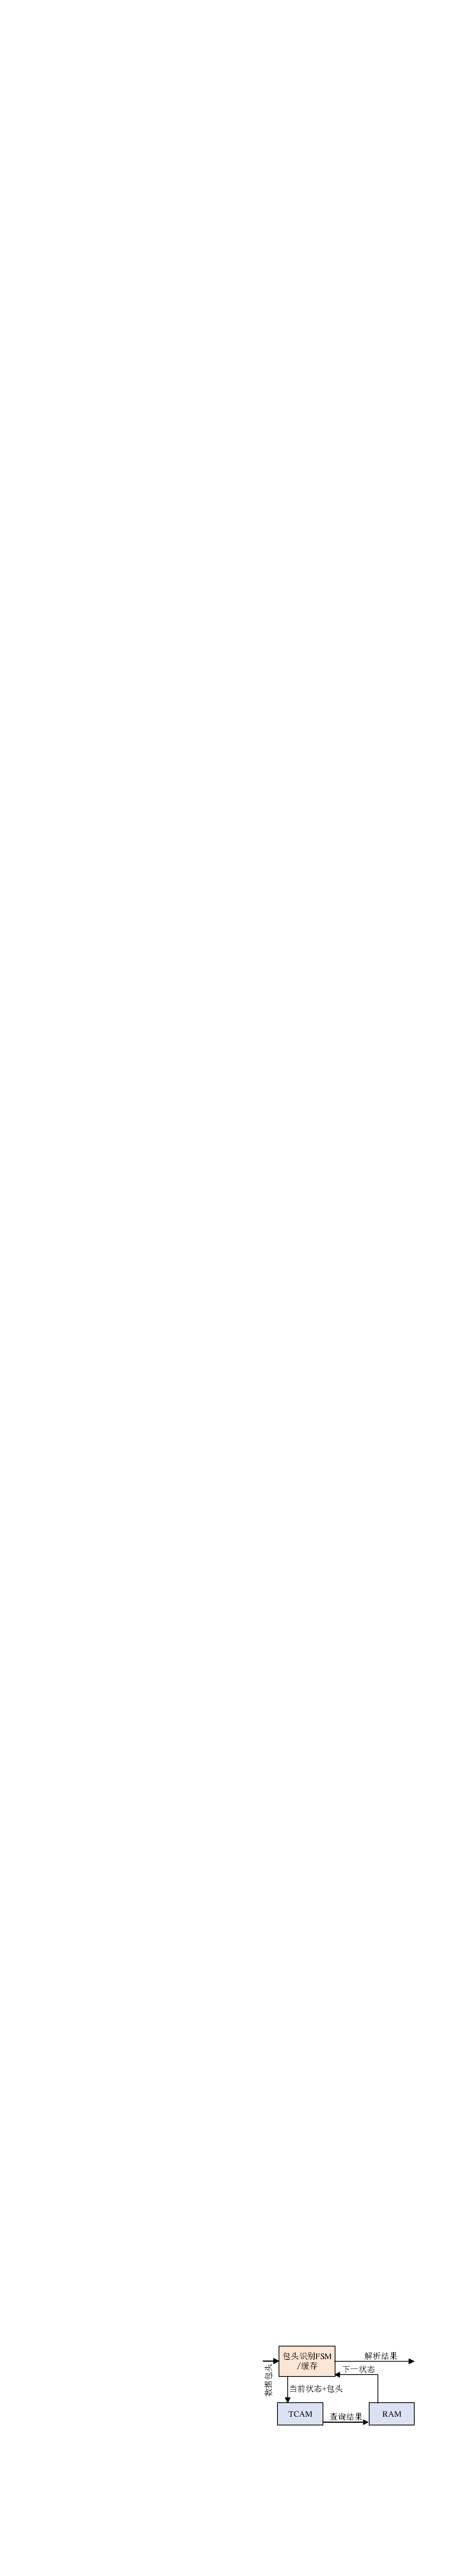
\includegraphics[scale=1]{progparser.pdf}
		\caption{基于ASIC的可编程包头协议解析器架构} \label{fig:progparser}
	\end{minipage}
\end{figure}



可编程包头解析器可以实现数据平面对新协议的可编程性。交换机中的查找表必须查找固定协议字段,所以每个交换机都会包括一个包头解析器,它能够标识当前数据包包头的协议名称。
如图~\ref{fig:pktheader}~所示,数据包是一组串行数据,从数据包的开始位置起,包头协议依次串行排列。每个协议段长度固定,每个协议末尾会有标识码标明下一个协议字段名称。本协议字段的长度一般都存储在协议字段内部。
图~\ref{fig:progparser}~所示为一种基于ASIC的可编程包头协议解析模型\citeup{gibb2013design},包头中的协议字段是一种有向图关系,图的节点代表协议,向量字段代表转移关系。
一个包的包头不一定包含图中所有的节点和对应关系,但当数据包到来时,包头所包含的协议只能是有向图中的唯一一种路径。一般使用有限状态机(FSM)就可以提取出包头内的所有协议字段。FSM内部存储完整的图关系,只要按照图对应关系来给包头不同字段打上协议名称标签即可。可见为了完成可编程的包头解析需要预先储备大量的查表资源,并且基于此的包处理器流水线的可编程能力是有限的\citeup{p4},依然不具备例如计算,状态转发,可编程触发等功能。

综上可见,目前最具有“高灵活性”的软件网络实现方案已经遇到了严重的性能瓶颈,而基于ASIC的网络数据平面编程能力仍然受到比较大的限制。网络数据平面的性能与可编程能力是一对看似矛盾的指标,目前如何提高基于硬件的网络处理器的可编程能力在学术界的研究成果还比较少。
 
  
   \ \ 

\BiSubsection{网络数据平面的编程抽象问题}{Programming Abstraction of Network Data Plane}\label{chap123}


{\hei 1)网络数据平面的全可编程抽象}


利用智能网卡来卸载操作系统内的网络功能,以期望获得比CPU更好的效能,同时还可以兼顾网络设计中不断变化的革新需求。智能网卡也称可编程网卡,相比于普通网卡:智能网卡不但可以完成网卡最基本的作用(主机与网络间通信),还应该有如下特征:输入输出多队列、TCP卸载、流量整形、规则过滤、虚拟化等\citeup{shinde2013we}。从而增强一些通用场景下的网络性能:带宽扩容、优化QoS(Quality of Service,服务质量)、降低CPU利用率、降低通信时延等。
随着时间的推移,研究人员还发现如果能够将计算\citeup{costa2012camdoop,sapio2017network}、随路功能聚合\citeup{mai2014netagg,graham2016scalable}、缓存\citeup{liu2017incbricks}甚至AI\citeup{sanvito2018can,innetworknn}都卸载到网络上,有能力显著提高分布式应用的处理效率。
目前能够支持这种将更复杂计算卸载到网络中的网卡,都要求有基于全可编程抽象的网络处理器或FPGA的智能网卡来实现。

基于网络处理器(Network Processor, NP)的数据平面,拥有完全的可编程能力\citeup{crowley2003network}。NP芯片内部一般包括基于硬件的拥塞控制、队列调度、QoS等协处理逻辑,还包括一组并行微码处理器。处理器按任务可分为核心处理器和转发引擎。处理器通过预先编制的微码来控制处理过程和内容。NP有通用的编程模式,一旦有新的技术或者需求出现,可以通过软件语义重新定义数据平面。值得注意的是NP中的众核一般使用数据平面专用精简指令集,为了达到节能与节约面积,例如浮点运算等复杂的处理指令是不支持的。NP的每个内核处理性能一般较差,NP的高性能需要结合使用专用外部电路,一旦处理的内容无法映射到专用电路,NP的性能优势会减弱\citeup{allen2003ibm}。另外,NP编程开发门槛较高,NP运行软件无操作系统扶持,并且代码移植性差,开发人员需要深入理解NP的处理模型,因此NP始终只在一些狭窄的领域空间内发挥作用。



基于FPGA的智能网卡拥有更为广阔的编程空间\citeup{firestone2018azure,putnam2017fpgas}。FPGA内部有大量LUT门电路,以及分布式片上互联网络,基于此结构的FPGA可以实现任何客制化的逻辑电路。文献\cite{wang2017p4fpga}将基于FPGA的智能网卡数据通路模型抽象化,利用高层次软件来编译硬件功能,可屏蔽底层数字电路设计细节,降低开发难度。FPGA可以方便地移植程序,设计人员可以将HDL代码打包成IP核,只要按照规定好的输入输出接口位宽和时序就可以任意复用。在设计电路模组时,一般会使用标准的总线接口来连接不同的功能模块,以增强开发的灵活性。如今FPGA厂商也会在FPGA中加入专用功能电路来增加芯片集成度、增强FPGA的处理某些任务时的性能,如ARM核、分布式DSP核、PCIe收发器、分布式片上存储。

{\hei 2)专用领域系统的可编程抽象}



为应对日益复杂的网络功能的可编程扩展,网络功能可编程需求增加。可编程系统提供专用领域所特有的特性是提升网络功能开发效率的重要手段。高级的专用领域可编程抽象可以大大降低开发人员的编程难度。对于流匹配的可编程思想,SDN抽象出对流表配置的可编程\citeup{mckeown2008openflow},P4抽象出了对流定义的编程\citeup{p4}。
在数据中心内,网络的管理很复杂,需同时考虑流量控制,拥塞控制,访问控制,攻击探测等诸多网络功能的实现。



%{\hei 2)网络测量性能可扩展性不足}
网络测量是实现上文功能的底层核心方法,在性能方面有极大的需求\citeup{d2019survey}。流量控制,拥塞控制需要利用网络流量实时速度以及平均包大小等相关信息,访问控制和攻击探测也需要用到流触发的反馈测量机制\citeup{zhang2018adaptive}。基于被动触发的网络测量系统是一种典型的测量实现技术,测量过程一般分为1)捕获,2)统计,3)存储三大部分。这三点也是影响测量系统性能的关键因素。目前在可编程数据平面中,支持可编程实现的网络测量技术限制于以基于CPU或网络处理器的平台。其性能受到CPU架构访存与计算能力的制约,每核心单独处理统计量能力在10Gbps以内\citeup{estan2004building,tahaei2017multi,hu2013discount},相比于通用服务器目前上百Gbps的吞吐需求,显然存在比较明显的性能弱势。一方面由于目标流量数目庞大,基于CPU架构的快速缓存空间不足,多级存储结构带来复杂的更新机制并且受限于外存储的非连续地址访问速率(<1Mpps\citeup{linux2020andree,bernat2017performance,yang2016rethinking}),性能表现力不稳定\citeup{einziger2017tinylfu}。另一方面,CPU计算架构过于通用化,反而在处理简单重复的重任务时无法发挥优势,尤其针对流式数据处理,CPU无法建立起可编程的高效率的流水线结构,严重制约了网络功能处理能力的可扩展性\citeup{tone2009network}。


综上所述,现代高性能网络正在向软件定义化、数据平面可编程的方向发展。可编程网络架构设计的核心,是构建一种支持映射高层次控制逻辑的数据平面。通过分析目前已有的工作内容,凝练出以下研究现状的不足之处:可编程网络的设计思想目前依然受到核心运算资源不足的限制,以及在工程实践中遇到可编程能力与吞吐性能之间的矛盾等问题,这为本文研究方向指明了道路。下一小节将介绍本文的研究内容主要以解决流表资源问题为基础,利用可编程硬件分别在网络中间节点、主机侧网络中构建了提升可编程性的方法,并形成一套完整的端到端系统。


\BiSection{论文研究内容与创新点}{Thesis Research Content and Innovation}\label{chap13}



\BiSubsection{研究挑战}{Research Challenges}\label{chap131}

综合以上研究工作可知,在数据平面的研究中,依然存在由于运算资源不足而导致的网络安全威胁问题,全可编程数据平面性能不足的问题。因此可编程网络数据平面的研究面临以下挑战:

{\hei 1)大规模流量场景下的流表资源扩展。}
研究软件定义网络下流表核心资源的供需关系以及调度问题,对保障交换机转发稳定性以及解决网络数据平面运算资源有限的问题有重要意义。
流表作为网络转发设备的核心资源有性能强、容量小等特征\citeup{qiao2016taming}。
软件定义网络作为可编程网络的经典范例,其对流量的精细区分更加导致流表容量不足,因而在软件定义网络场景下流表的容量问题变得更加凸显\citeup{kannan2013compact,qiao2018openflow}。
由于软件定义网络中建立流转发的行为需要远程控制器的支持,因此一旦流表溢出发生数据平面将会对控制平面产生源源不断的流表项建立查询请求,严重情况下会导致控制通道拥塞,进而影响网络其他控制进程,最终导致网络转发功能失效\citeup{zhouyadong2017liubiao}。
依靠增加流表容量的方式可以降低流表溢出的风险概率,但不会对缓解流表溢出后系统安全问题产生实质性的解决,目前研究领域对问题此尚无成熟的技术以及方法。

{\hei 2)数据驱动网络下计算与转发协同优化。}
研究可编程网络场景下融合计算与通信的协同优化方法,对解决网络数据平面的可编程能力有限的问题具有重要意义。
虽然软件交换机在网络编程能力以及可编程计算领域方面大幅超过硬件交换机,随着CPU处理性能增速放缓,以及网络数据包吞吐容量迅速增大,其性能较弱的特点已经成为阻碍可编程网络发展的重要瓶颈\citeup{ge2014openanfv,li2018dhl}。
基于P4可编程芯片的网络交换机虽然性能足够强大,但是其可编程空间比较小,缺乏对复杂计算需求的支持\citeup{wang2017p4fpga}。
如何在硬件环境下解决网络设备灵活性与高性能直接的矛盾,目前依然是一个开放性问题。

{\hei 3)新型编程抽象模型下网络硬件资源受限。}
研究可编程网络的编程抽象方法,并保障相应的高性能硬件资源占用约束,对提升高性能网络功能开发效率以及构建细粒度流量的网络功能具有重要意义。
在当前数据中心内,实现灵活多变的网络功能主要通过服务器软件方式,虽然软件具有快速部署的特性,但在实现网络测量领域功能时,软件处理高时间精度的能力较低\citeup{qiao2014network}。
同时,面对大量并发触发的网络测量任务,CPU系统的能效比已经处于劣势\citeup{liu2019e3,le2017uno}。
如何利用资源有限的网络数据平面中的可编程硬件,并在其之上建立一套针对网络测量领域的可编程网络系统,目前尚待进一步研究。

\BiSubsection{本文研究内容与创新点}{The Research Content and Innovation of the Article}\label{chap132}
%本文主要
本文以解决流表瓶颈资源问题为基础,研究在网络数据平面内如何利用可编程硬件来更灵活、更高效地支持多种类别的可编程抽象方法。
针对高性能网络以及数据平面可编程领域内的三个挑战,本文利用可编程硬件分别在网络中间节点、主机侧网络中构建了能够同时提升设备性能以及灵活性的方法,最终构成一套完整的端到端网络系统。

\begin{figure}[!ht]
	\centering 
	\vspace{-1.5mm} 
	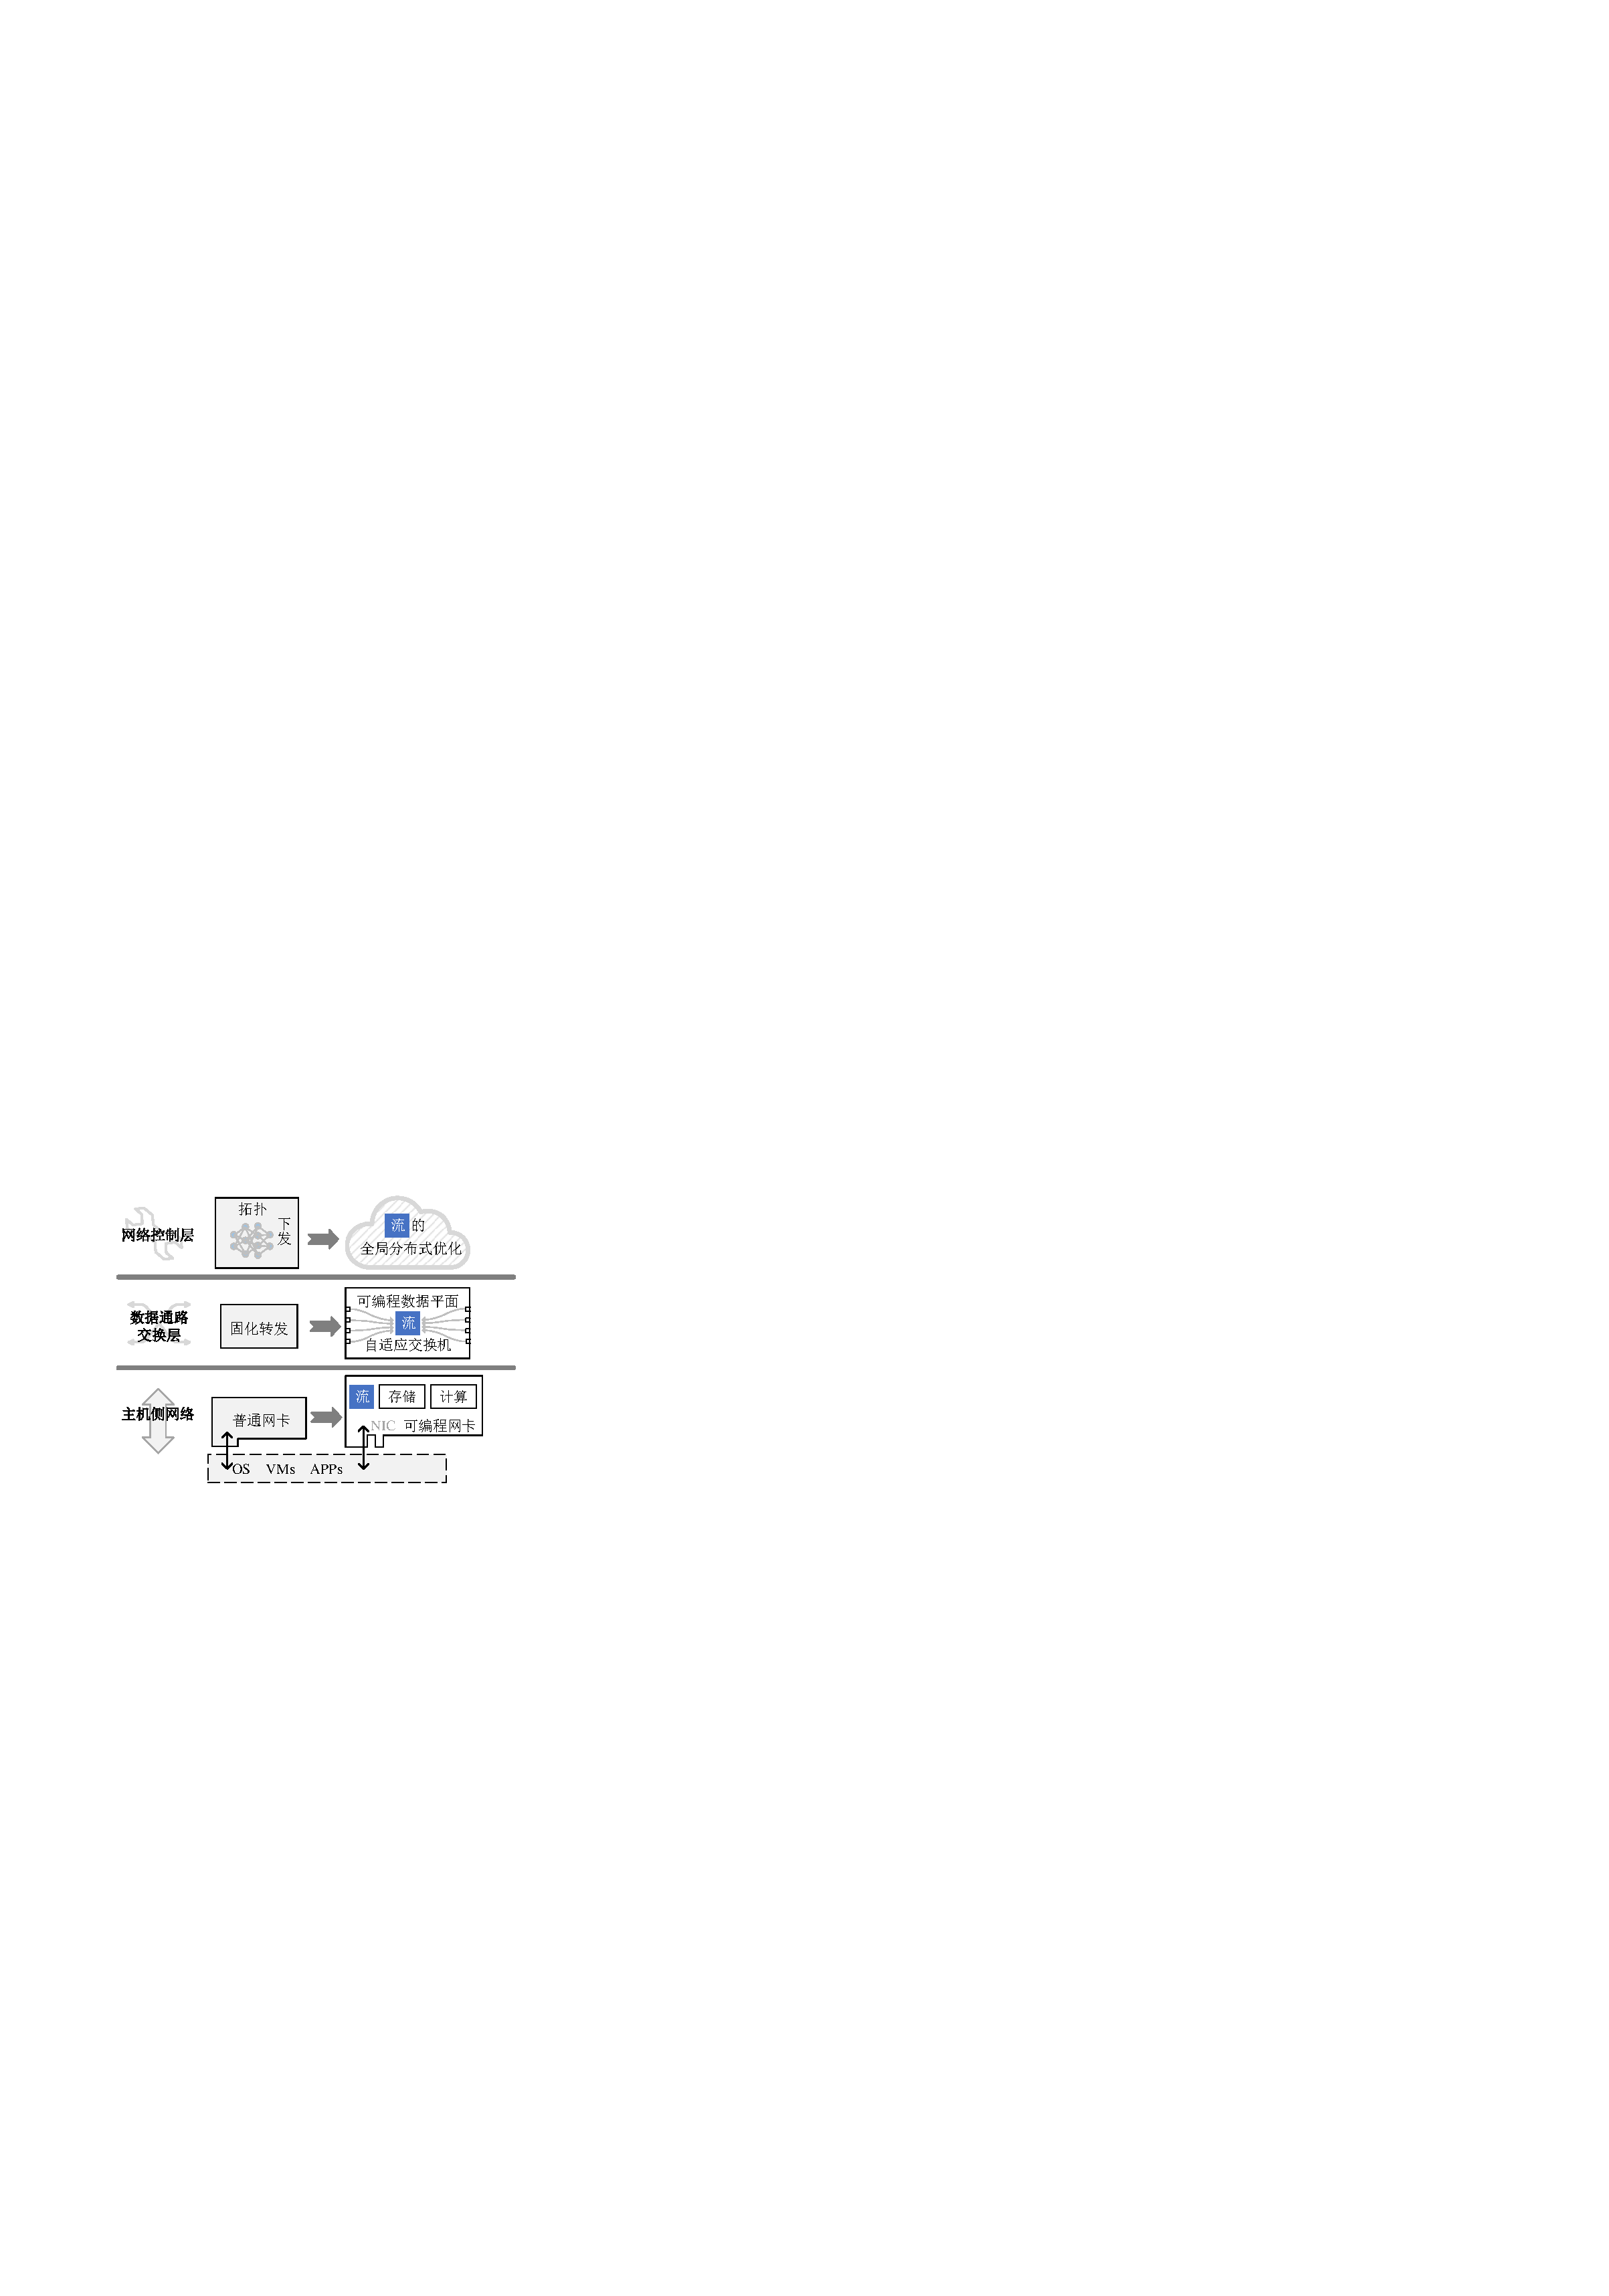
\includegraphics[scale=1]{proghardwarePDParcs.pdf}
	\caption{基于可编程硬件的SDN数据平面研究框架} \label{fig:proghardwarePDParcs}
\end{figure}

如图~\ref{fig:proghardwarePDParcs}~所示,本文从网络的三个层次出发,对可编程网络在每一个层次内做了改进。
首先,流表是基于硬件的高性能数据包转发的核心资源,在研究内容一中利用软件定义网络控制平面高可配置性,对数据平面的流表资源进行了全局优化。
其次,利用可编程硬件与交换芯片结合的异构结构,在研究内容二中设计一种自适应交换结构,优化数据平面网络节点的可编程能力。
第三,针对主机侧网络中基于网络测量的网络功能,研究内容三提出了统一的软硬件结合编程抽象方法,利用硬件可编程网卡实现了高性能、高精度以及高效率的网络功能可编程系统。


具体研究内容概况如下:

{\hei 研究内容一:软件定义网络内交换机硬件流表可扩展性研究(第~\ref{chap5}~章)}

{\hei 本文从SDN网络全局视野出发,着手解决流表资源匮乏的问题。}
由可编程网卡和交换机组成的数据平面内,流表资源是提升设备性能的核心,网络数据包的转发动作依赖于数据平面内查找表的匹配结果,在此基础上交换机内还增加了多种匹配域、多级流表结构,绝大多数平台中都视转发表为最核心以及成本占用最大的模块,软件定义网络(SDN)架构下亦是如此。
基于硬件的高性能TCAM\citeup{katta2014infinite}(三态内容地址查找表)拥有单周期流水、掩码匹配等优秀性能,但昂贵的价格使得用户无法购置容量足够大的表\citeup{kuzniar2015you},因此交换机内极易发生流表溢出的现象。
以OpenFlow协议为代表,一般规定控制器与交换机之间流表安装流程为Reactive模型:交换机收到一条新流首先会上报控制器,随后控制器计算路径并下发流表到数据平面设备。
当发生流表溢出现象时,由于Reactive模型需要频繁更替活跃流表内容,这会进一步直接引发控制平面和数据平面之间安全通道的消息风暴,否则会造成丢包或服务任务中断等异常现象。
第一个研究内容下有两个子问题:如何在维持交换机中原有流表容量的前提下,缓解流表溢出所带来的危害?在保持SDN网络平面分离优点的条件下,如何利用其全局化优势高效利用网络设备资源?


{\hei 创新点:}本文分析不同的流量规模和特征,以及系统多模块之间的互联协议,提出一种转发设备节点之间的流表共享机制(Flow Table Sharing, FTS)。

1)为保障控制平面免于遭受大量突发服务请求,FTS实现了一种离线转发策略,同时减轻了安全通道的通信压力。实现了在流量突发的情形下,保证数据平面稳定性,降低SDN系统控制通道拥塞、失效风险,缓解流表溢出导致转发性能骤降的现象。

2)为保障数据平面流表资源充足,本文分析并修改了目前OpenFlow协议中有关Table-Miss(流表缺失状态)的处理过程,并修改了OpenFlow协议中关于未知数据包上报条件,在数据平面内利用交换机组表进行聚合转发,并且可以方便地退回现有规范。

本文论证了单纯依靠增加流表容量的方案,并不能使流表溢出的概率降低为零,并且能够容易回退、向下兼容现阶段的传统方案。FTS通过通过增强数据平面自主性等方法,在流表溢出的情况下,该方案和传统OpenFlow协议相比,使OpenFlow交换机转发RTT延迟和安全通道控制报文风暴数量的优化均达到至少2个数量级。



{\hei 研究内容二:可编程设备增强网络交换节点计算能力的研究(第~\ref{chap4}~章)}

{\hei 本文从网络数据平面处理器的底层设计出发,在现有的大规模集成电路设计能力的基础上,构建可行的网络处理器流水线模型。}
由于新兴的内容应用(社交,虚拟/增强,混合现实)以及工业网络应用(移动性,大数据,机器学习)使得网络追求高的实时性、可扩展性。
网络设备功能多样性随着数据中心、边缘设备的发展而壮大,因此学界对交换层、核心网场景下快速创建灵活解决方案的需求也愈发强烈。
可编程数据平面交换机的三类典型设计架构但目前都存在缺陷:1)软件交换机性能普遍低下,2)基于ASIC的交换机无法拥有完全可编程性,3)基于FPGA的交换机资源有限,交换性能无法满足业界需求。
本文研究内容首先提出一种新型的可编程网络数据平面,采用异构设计的思想,解决上述典型设计的缺陷。
因此本文第二个研究问题:如何设计一种同时兼顾转发性能和可编程能力的交换设备?如何利用现有设备优势,对其做最小改动以满足设计?如何实现高资源利用率、高灵活性的高性能硬件可编程数据平面设计方法?

{\hei 创新点:}本文提出一种高性能的数据平面可编程硬件架构,自适应交换结构(Adaptable Switch, AS)。

1)为同时增强AS架构的灵活性和吞吐性能,AS提出一种旁路数据处理流水线模式。通过FPGA与交换芯片联合设计的思想,AS架构可同时提供FPGA的高灵活性与交换芯片的强大性能。论文在前述硬件设计模型的基础上,继续研究硬件逻辑高度并行的性能大规模扩展方法。

2)为增强可编程硬件内的数据处理吞吐能力,AS架构设计了一种资源占用低的流量均衡式并行处理模型。

3)为增强AS架构控制平面的处理性能,本文设计了一种高效的启发式流表分配算法。AS架构解决了FPGA性能差与资源少的限制、增强了网络芯片的可编程能力,并且提出了一套部署在硬件上的高资源利用率的并行流水线和流表分配优化算法。

论文设计了ASIC面向可编程硬件的扩展接口。交换芯片将数据包头拆分并通过高速数据互联载体发送给FPGA,利用FPGA可重配特性实现完全可编程的包头处理。自适应交换系统在满足全可编程灵活性的条件下,与基于FPGA的数据平面相比,将数据包处理性能提升120倍以上\footnote{当前的研究中,主流全可编程目标平台性能约为60Gbps。}。

{\hei 研究内容三:端侧网络的网络测量领域内可编程研究(第~\ref{chap3}~章)}

{\hei 本文提出利用基于FPGA的智能网卡卸载操作系统内网络测量任务,通过软件配置的方式,令系统硬件支持高性能的网络安全、访问控制、拥塞探测、流量控制等多种场景。}
目前可编程网络领域缺乏对以上偏向底层的网络功能的统一抽象,开发人员需要独立实现功能细节,重新开发某些通用模块,耗费大量的人力物力。
许多网络应用的基础是实现网络测量任务,本文将测量过程分解为三类子操作,1)捕获;2)统计分析;3)流量发送。捕获数据包时需要对每个数据包添加时间戳等数据记录工作,以供流量离线分析以及在线分析使用。
在线统计分析对高性能和高实时性的特性要求极高。
分析后的流量需要按原始流量顺序与速率再向网络接口发送回去。
其中统计分析模块是可编程网络测量系统的核心模块,目前基于FPGA硬件可编程网卡同时提供了高性能收发和足够强大的灵活性已经可以满足主机侧网络的性能需求,为更复杂功能的卸载提供了有力支持\citeup{alveo250,netfpgaabout}。
如何利用可编程网卡实现高精度、高性能保障和高能源效率的网络功能硬件卸载?提出测量功能可编程抽象、合理部署和划分任务是本文要解决的问题。

{\hei 创新点:}
网络测量是众多网络功能的基础,本文针对目前为了功能应用提出了统一的编程抽象方法。

1)为提升网络功能的编程灵活性,本文将针对网络测量领域的编程方式抽象为统计、触发模型。上层软件通过灵活调用测量数据来做更高层次的网络测量应用,令系统硬件适用于高性能的网络安全、访问控制、流量控制、拥塞探测等多种场景。

2)为增强终端可编程网络节点的性能,本文本文提出了一套基于智能网卡的硬件流水线系统,包括数据包捕获功能、测量系统和发送引擎。本文将其中测量系统操作抽象为基础的包个数统计和数据量缩统计方法。

3)为增基于测量的可编程网络抽象的可用性,本文本文提出一种基于硬件的存储压缩的无偏估计算法,在节约38\%的硬件存储空间情况下,相较于软件的处理方式系统吞吐率提升8倍、系统的处理能耗节约90\%。



如图~\ref{fig:thesistree}~所示,将本文的主要研究内容以及研究成果结构化地展示出来。


\begin{figure}[!ht]
	\centering 
	\vspace{-1.5mm}
	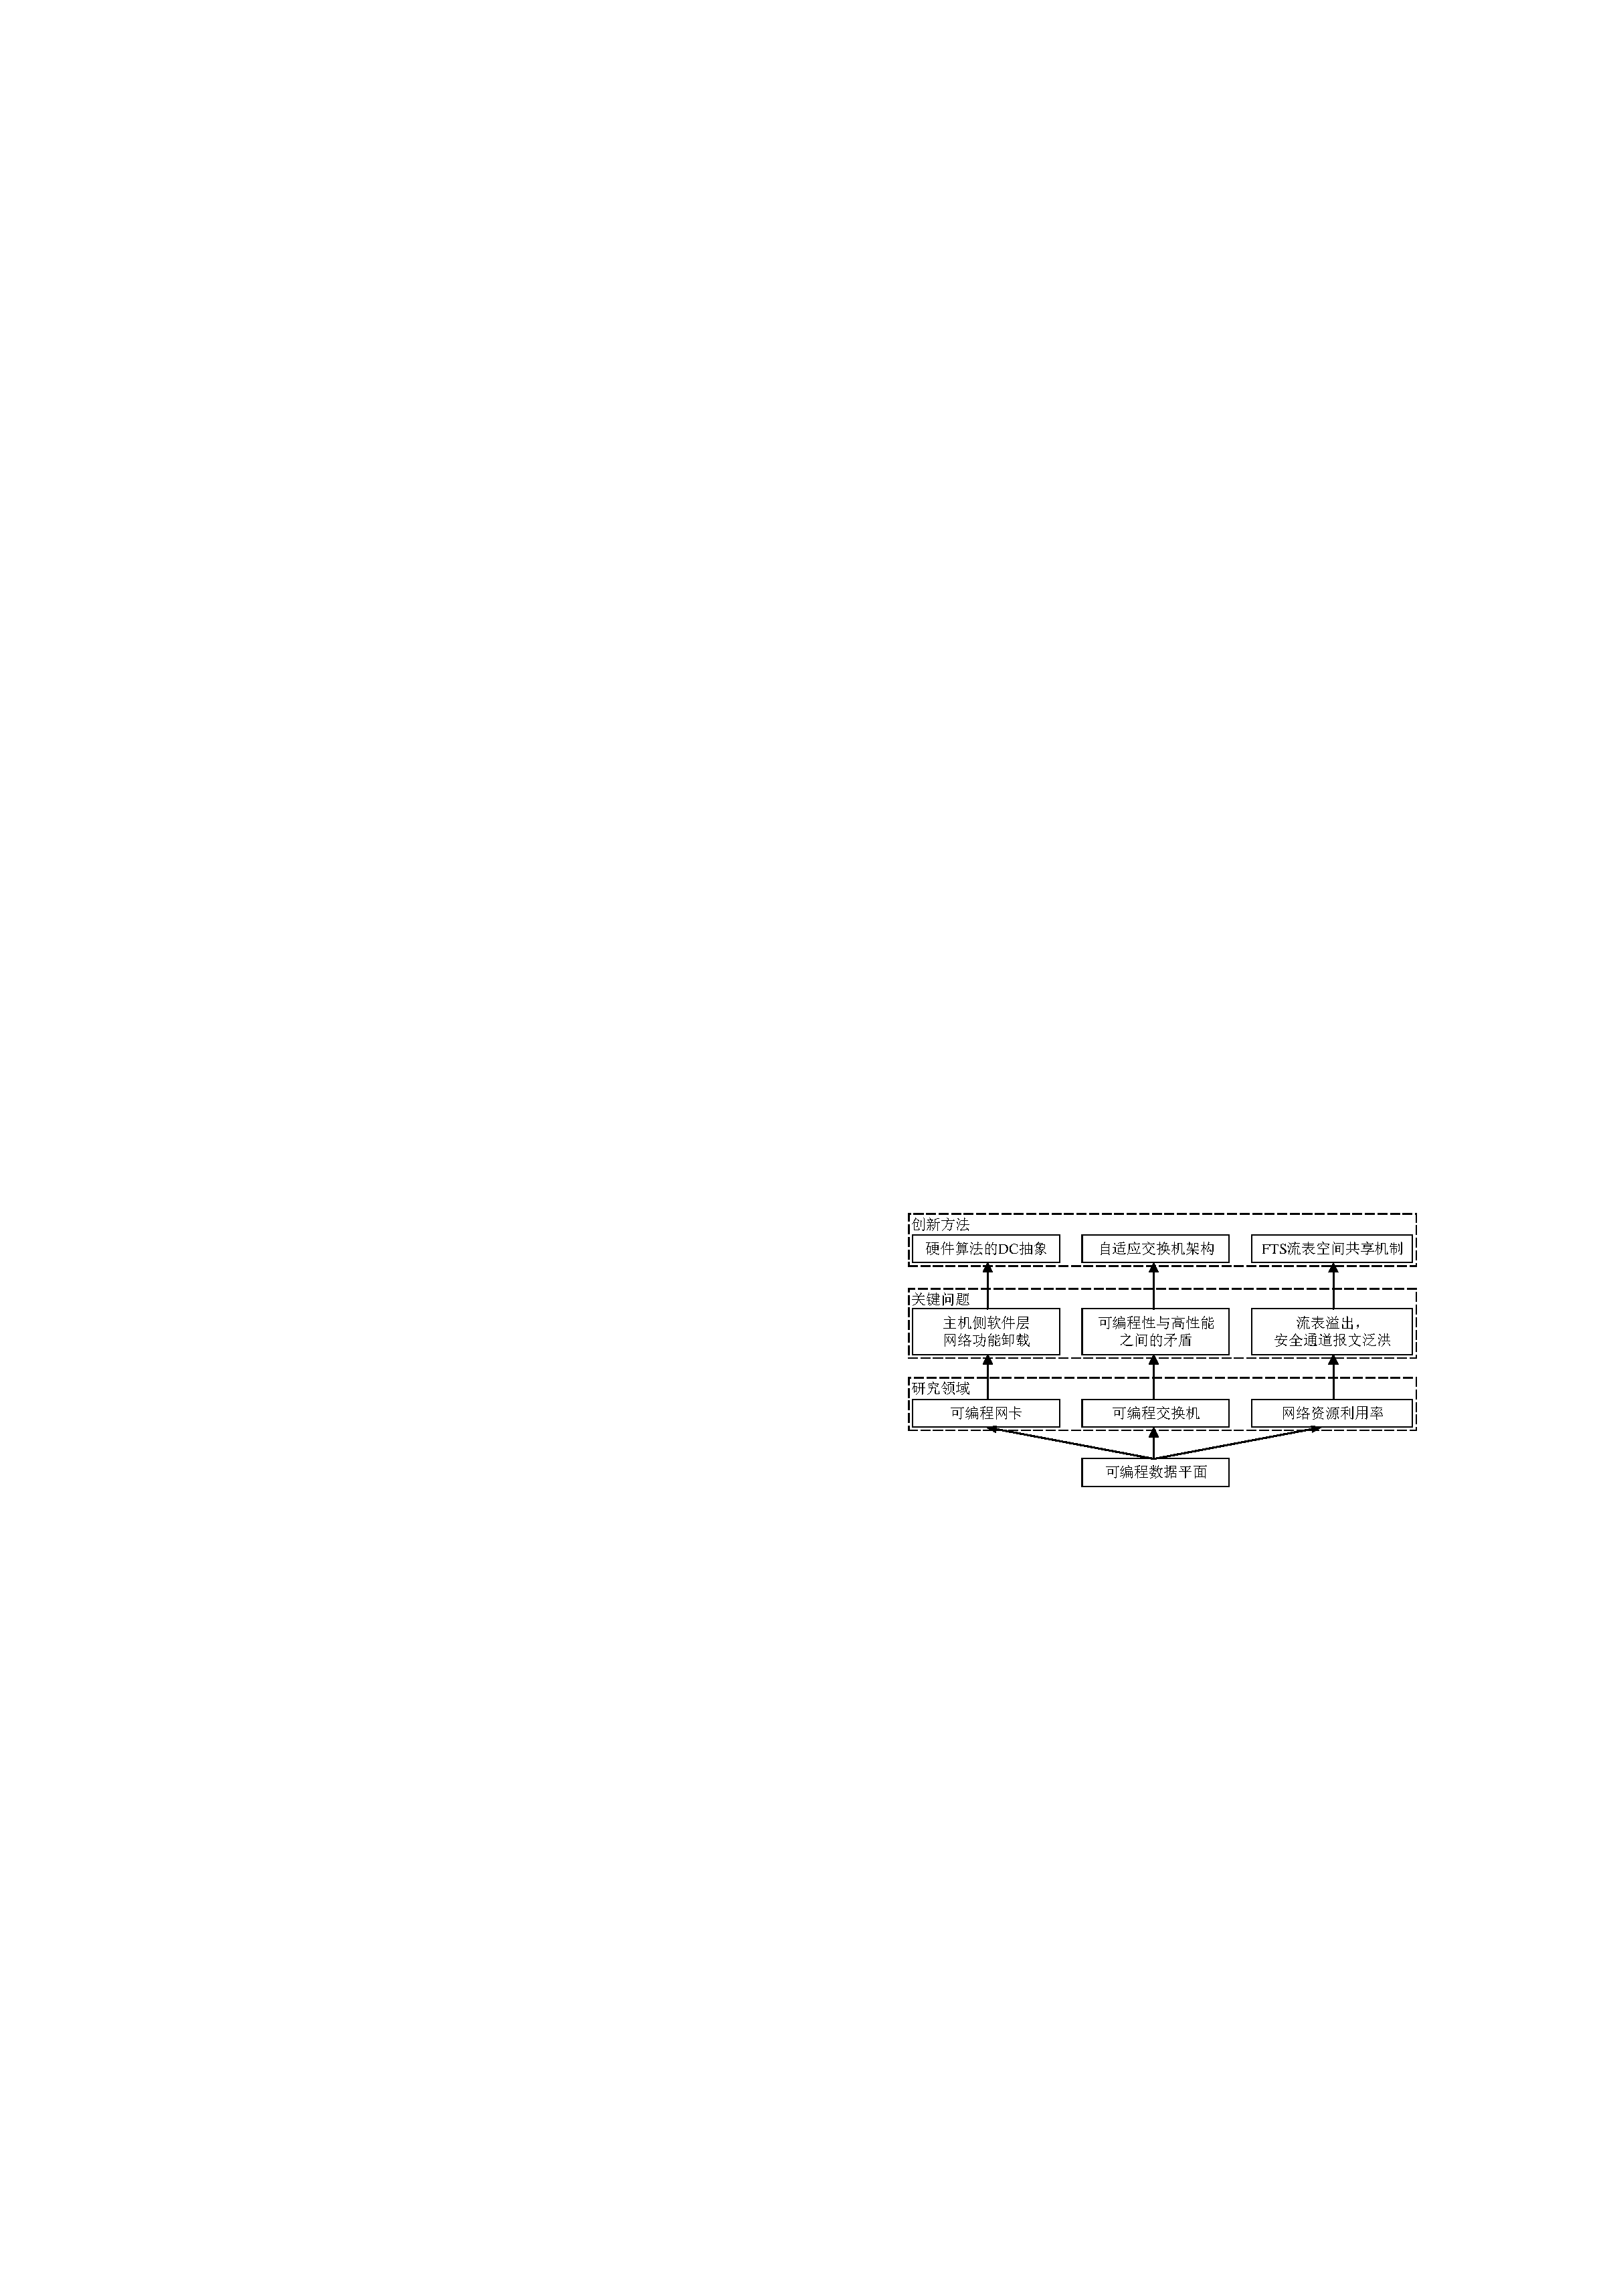
\includegraphics[scale=1]{thesistree.pdf}
	\caption{论文主要研究内容以及成果} \label{fig:thesistree}
\end{figure}







\BiSection{论文组织结构}{Organization of the Thesis}\label{chap15}

论文共分为五个章节,具体组织结构安排如下:

第~\ref{chap1}~章为绪论,主要讨论研究背景、相关工作综述,分析可编程网络硬件的发展方向、目前研究所面临的挑战以及总述全文。本文接下来三章内容主要针对绪论提出的挑战而做出深入的研究。
%第\ref{sec:pdpintro}章为。

第~\ref{chap5}~章主要对网络数据平面内的流表资源做可扩展研究,提出一种全局优化方法来改善流表溢出带来的安全性风险。

第~\ref{chap4}~章论述一种FPGA与交换芯片相结合的异构网络数据平面硬件架构,令交换机系统拥有灵活的可编程能力的同时,处理吞吐性也能得到显著提升。

第~\ref{chap3}~章论提出了一种高资源利用率的针对网络测量领域编程抽象,通过不同的软件调用,令系统硬件专用处理器适用于高性能的网络安全、访问控制、流量控制、拥塞探测等多种场景。

第~\ref{chap6}~章总结全文工作,并展望未来研究方向。




































%-----------------------------------------------------------------------------------------
%\BiSection{为什么用 \LaTeX}{Why}
%
%虽然论文排版是一项基本技能,但是从实际情况看,同学们经常被各种格式整得晕头转向。加之 Word 排版不够美观,版本管理麻烦,排版效率低下,因此开发 \LaTeX{} 论文模板非常重要。国际上许多著名的出版机构和学术期刊都有自己的 \LaTeX{} 模板,国内外许多高效也有自己的硕博论文 \LaTeX{} 模板。事实上,\LaTeX{} 已经成为科技出版行业的国际标准,特别是数学、物理、计算机和电子信息学科。
%
%采用 \LaTeX{} 排版主要有以下优点:
%\begin{enumerate}
%	\item 排版质量高:主要体现在对版面尺寸的严格控制,对字距、行距和段距等间距的松紧适度掌握,对数学公式的精细设计,对插图和表格的灵活处理,对代码和算法的优美呈现,等等。
%	\item 安全稳定:自发布以来 \TeX{} 和 \LaTeX{} 没有发现系统漏洞,不会出现死机或者系统崩溃而导致编写的内容来不及保存。
%	\item 灵活方便:\LaTeX{} 的源文件是纯文本文件,文件大小比 Word 小很多,不会因为文容的增加而导致文档打开、编辑、保存和关闭等操作变慢。因为 \LaTeX{} 在编译时才将所有源文件和图表汇总,故撰写内容时可以随意增删章节和图表。并且和大部分程序设计语言一样,\LaTeX{} 具有注释功能,作者可以在源文件任何地方添加注释,而不会影响最终生成的文档。
%	\item 格式和内容分离:\LaTeX{} 将文档格式和文档内容分开处理,作者只要选择合适的模板,就可专心致志地撰写文档内容,文档的格式细节则由 \LaTeX{} 模板统一规划设置。特别是文献管理能力非常强大,这给撰写像博士论文一样需要大量引用参考文献的文档提供了很大便利。
%	\item 免费开源:\LaTeX{} 软件完全免费,源代码也全部公开,并且相应的配套软件也都采用开源的方式。
%\end{enumerate}
%
%无论你是因为羡慕 \LaTeX{} 漂亮的输出结果,还是因为要给学术期刊投稿而被逼上梁山,都不得不面对这样一个事实:\LaTeX{} 是一种并不简单的排版软件,不可能只点点鼠标就弄好一篇漂亮的文章。还得拿出点搞研究的精神,通过不断练习,才能编排出整齐漂亮的论文。一旦你掌握了如何使用 \LaTeX{} 撰写出精美漂亮的论文时,你会发现你的决定是明智的,你的投入是值得的。
%
%%=========================================================================================
%\BiSection{怎样用 \LaTeX}{How} 
%
%本模板在 Windows + TeXLive2016 + Texsdudio 平台下开发,采用 XeLaTex 编译。虽然之前也开发过一个基于 CTeX 的模板,但是经过多方面比较发现 TeXLive+XeLaTex 处理中文更好,所以基于 CTeX 的模板没有共享。
%
%{\color{red}本模板不能在 CTeX 软件下使用,必须采用 TeXLive,并且编译方式是 XeLaTeX。TeXLive 每年更新一个版本,我用的是 TeXLive2016。文本编辑器可以根据自己的喜好选用,我用的是 Texsdudio,这款开源软件非常不错,推荐大家使用。}
%
%本模板的源文件通过主目录下的 main.tex 统一管理,setup 文件夹中存放格式定义和封面、摘要、目录等内容,body 文件夹中存放论文正文章节的源文件,appendix 文件夹中存放附录、致谢和声明等内容。
%
%本模板只提供论文的格式定义,不提供 \LaTeX{} 的详细使用方法。%所以只回复和论文格式相关的问题,不解答具体的排版方法和技巧。
%因为 \LaTeX{} 的资源非常丰富,大家可以在网上查找资料和并参与讨论,这样学习效率更高。我关注的两个网站是:\url{http://bbs.ctex.org/forum.php} 和 \url{http://www.latexstudio.net};参考的两本书是 ``The Not So Short Introduction to \LaTeXe'' 和 ``LaTeX2e完全学习手册''。
